\section{Qualitative Analysis and Visual Interpretability}

\subsection{Visual Attention Verification in Sub-Problem 1}
To verify that Stage 1 ConvNeXt-Tiny vehicle count regression grounds its predictions in physical vehicle visual features rather than background environmental shortcuts (such as road markings, tree shadows, or weather glare), we analyze feature attribution maps using visual attention visualizations.

Figure~\ref{fig:attention_map} presents attention heatmaps generated by the ConvNeXt-Tiny vehicle counting model across representative traffic camera scenes.

\begin{figure}[htbp]
\centering
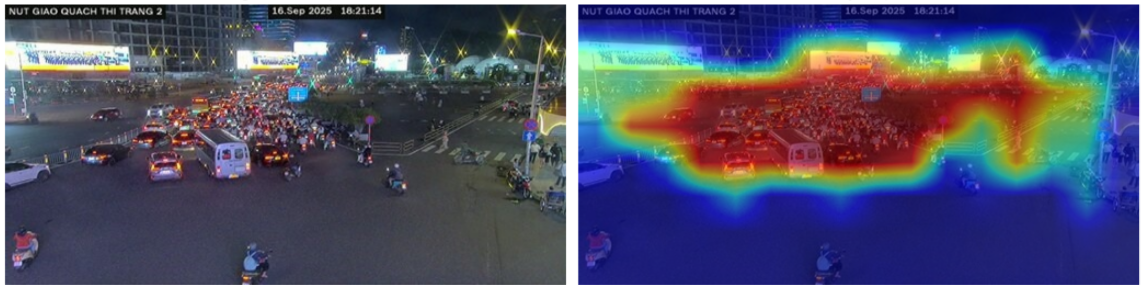
\includegraphics[width=\columnwidth]{fig/attention_map.png}
\caption{Visual attention heatmaps generated by ConvNeXt-Tiny vehicle count regression model, confirming high attention focus on vehicles (motorbikes and cars) in camera feeds.}
\label{fig:attention_map}
\end{figure}

The attention heatmaps demonstrate that ConvNeXt-Tiny concentrates high attention weights directly on active vehicle clusters (passenger cars and motorcycle streams). The $7 \times 7$ depthwise receptive fields effectively isolate vehicle regions even under partial occlusions and high traffic density, confirming that direct regression learns genuine visual representations of vehicle presence.

\subsection{Temporal Self-Attention Analysis in Sub-Problem 2}
In Stage 2 \textbf{TA-STGCN}, the Model-Level Multi-Head Temporal Self-Attention layer computes dynamic attention weights $\mathbf{A} \in \mathbb{R}^{T_{\text{in}} \times T_{\text{in}}}$ across historical time steps ($T_{\text{in}} = 24$, corresponding to 120 minutes of observation).

During peak morning and evening rush hours, the attention weights dynamically focus on recent time steps ($t-1$ to $t-4$, corresponding to the last 20 minutes) as well as periodic steps ($t-12$ and $t-24$, corresponding to 60 and 120 minutes prior). This confirms that TA-STGCN dynamically combines recent temporal momentum with periodic daily patterns to predict impending congestion build-up across the 608-node road network.
